\subsection{Load Store Unit}

\begin{figure}[H]
    \centering
    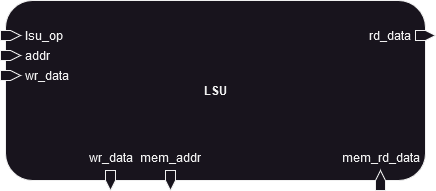
\includegraphics[width=0.5\textwidth]{../diagrams/memory/lsu.png}
    \caption{Load Store Unit}
    \label{fig:lsu}
\end{figure}

The LSU is a module that is responsible for memory access. It will manage the different READ and WRITE to the memory and for example
mask the data you want to read or write according to the given instruction.

Signals:
\begin{enumerate}[label={\textbullet}]
    \item Input: $lsu\_op$, This signal is representing the type of memory access you want to perform.
    \item Input: $addr$, This signal is representing the address of the memory you want to access.
    \item Input: $wr\_data$, This signal is representing the data you want to write to the memory.
    \item Input: $mem\_rd\_data$, This signal is representing the value that has been read from the memory.
    \item Output: $wr\_data$, This signal is representing the value that should be written to the memory and correctly
    masked according to the given instruction.
    \item Output: $mem\_addr$, This signal is representing the address you want to write or read to the memory.
    \item Output: $rd\_data$, This signal represents the value that has been read from the memory and correctly 
    masked according to the given instruction.
\end{enumerate}